\newpage
\appendix


\renewcommand{\thepart}{}
\renewcommand{\partname}{}

\part{\huge{\textbf{Appendix}}} % Start the appendix part
\parttoc % Insert the appendix TOC
\clearpage


\section{Google Research Football (GRF) Tasks Setup}
\label{app:grf}

\begin{figure}[h]
    \centering
    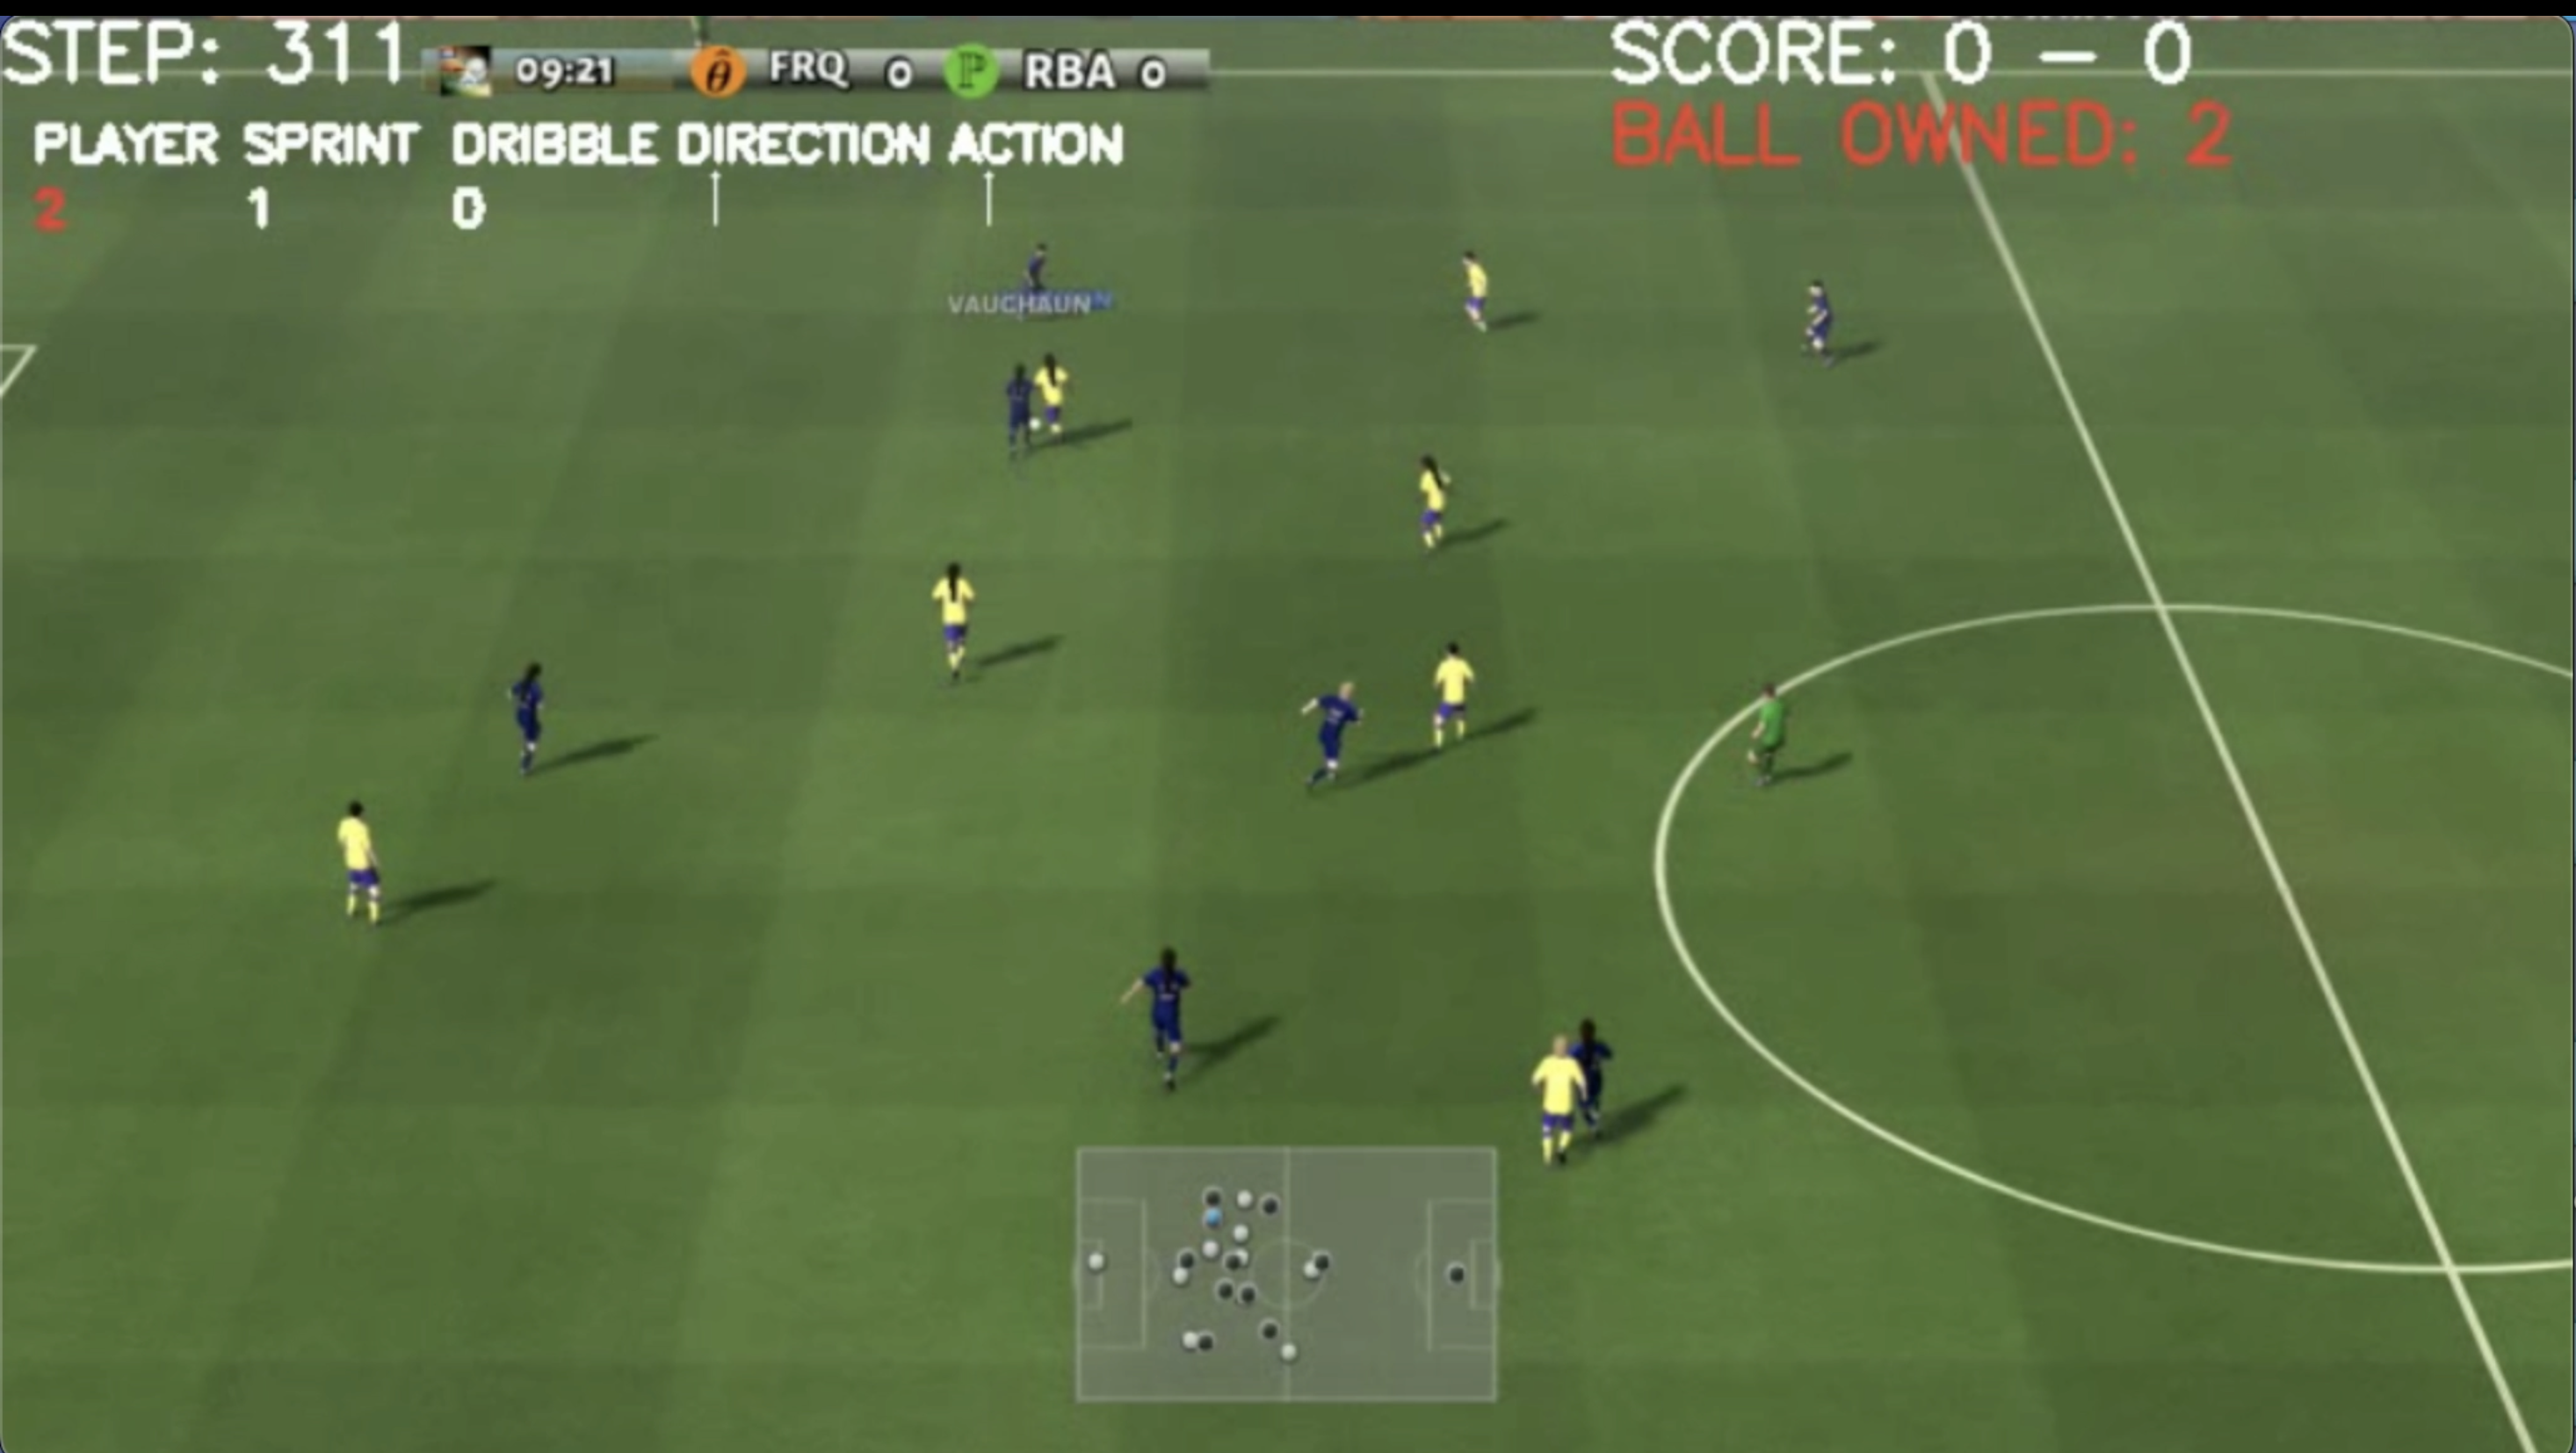
\includegraphics[width=0.75\textwidth]{fig/football_main.png}
    \caption{Illustration of the game in football simulator.}
    \label{fig:football_main}
\end{figure}


In this section, we mainly focus on the GRF implementation\footnote{https://github.com/google-research/football/blob/master/gfootball/} and the modifications we made under this environment. 
\subsection{State Space}


The raw state of each player contains information about the game state, the ball and all players on the pitch. The game state includes scores, game modes indicating free kicks, corner kicks or other game stages, and game time represented as steps. The ball information includes its spatial position, direction, and an indicator for ball ownership (identifying the player and team that possess it). The player information comprises position, direction, roles, yellow card records, and more. For players on the opposite team, positions and directions are mirrored. The details of the raw state are as follows:

\begin{itemize}[leftmargin=*]
\item \textbf{Ball Information:}
\begin{itemize}
\item \texttt{ball} -- $[x, y, z]$ position of the ball.
\item \texttt{ball\_direction} -- $[x, y, z]$ ball movement vector.
\item \texttt{ball\_rotation} -- $[x, y, z]$ rotation angles in radians.
\item \texttt{ball\_owned\_team} -- \{-1, 0, 1\}, where -1 indicates the ball is not owned, 0 denotes the left team, and 1 the right team.
\item \texttt{ball\_owned\_player} -- \{0..N-1\} integer denoting the index of the player owning the ball.
\end{itemize}

\item \textbf{Left Team:}
\begin{itemize}
\item \texttt{left\_team} -- N-elements vector with $[x, y]$ positions of players.
\item \texttt{left\_team\_direction} -- N-elements vector with $[x, y]$ movement vectors of players.
\item \texttt{left\_team\_tired\_factor} -- N-elements vector of floats in the range \{0..1\}. 0 means the player is not tired at all.
\item \texttt{left\_team\_yellow\_card} -- N-elements vector of integers denoting the number of yellow cards a given player has (0 or 1).
\item \texttt{left\_team\_active} -- N-elements vector of booleans denoting whether a given player is playing the game (False means the player got a red card).
\item \texttt{left\_team\_roles} -- N-elements vector denoting roles of players, where:
\begin{itemize}
\item \texttt{0} = \texttt{e\_PlayerRole\_GK} - goalkeeper,
\item \texttt{1} = \texttt{e\_PlayerRole\_CB} - centre back,
\item \texttt{2} = \texttt{e\_PlayerRole\_LB} - left back,
\item [...]
\end{itemize}
\end{itemize}

\item \textbf{Right Team:} Same attributes as for the left team.

\item \textbf{Controlled Player Information:}
\begin{itemize}
\item \texttt{active} -- \{0..N-1\} integer denoting the index of the controlled players.
\item \texttt{designated} -- \{0..N-1\} integer denoting the index of the designated player.
\item \texttt{sticky\_actions} -- 10-elements vectors of 0s or 1s denoting whether a corresponding action is active.
\end{itemize}

\item \textbf{Match State:}
\begin{itemize}
\item \texttt{score} -- Pair of integers denoting the number of goals for the left and right teams, respectively.
\item \texttt{steps\_left} -- How many steps are left till the end of the match.
\item \texttt{game\_mode} -- Current game mode.
\end{itemize}
\end{itemize}

\textbf{For the imaginary dataset generation, we created our own Imaginary state}, which includes the following information:

\begin{itemize}[leftmargin=*]
\item \textbf{Game Information:}
\begin{itemize}
\item \textbf{Sticky actions:} A list of currently active sticky actions.
\item \textbf{Game mode:} The current game mode.
\item \textbf{Score:} The current score of the game.
\item \textbf{Time:} The current game time in minutes and seconds.
\item \textbf{Active player:} The index of the currently active player.
\item \textbf{Active player role:} The role of the currently active player.
\item \textbf{Ball ownership:} The team currently in possession of the ball (none, left team, or right team).
\item \textbf{Ball ownership player:} The index of the player currently in possession of the ball.
\item \textbf{Ball zone:} The zone where the ball is located.
\item \textbf{Ball direction:} The direction in which the ball is moving.
\end{itemize}

\item \textbf{Player Information:}
\begin{itemize}
\item \textbf{Team:} The team the player belongs to (left team or right team).
\item \textbf{Role:} The role of the player.
\item \textbf{Zone:} The zone where the player is located.
\item \textbf{Direction:} The direction the player is facing.
\end{itemize}
\end{itemize}


The imaginary state is designed to provide a more compact and informative representation of the game state compared to the raw state. It extracts and processes the relevant information from the raw state, making it easier to understand and use for generating imaginary data.

The sticky actions, game mode, score, time, active player, and active player role provide a high-level overview of the current game state. The ball ownership and ball ownership player indicate which team and player are currently in control of the ball. The ball zone and direction give spatial information about the ball's location and movement.

For each player, the Imaginary state includes their team, role, zone, and direction. This information helps in understanding the positioning and orientation of the players on the pitch.

By including these key pieces of information in the Imaginary state, we aim to capture the essential aspects of the game state that are relevant for generating realistic and diverse imaginary data. The imaginary state serves as a preprocessed and structured representation of the raw state, making it more suitable for the subsequent steps in the imaginary data generation process.

Here, we show an example of imaginary state,


\begin{bbox}{Imaginary State}
\begin{verbatim}
{'active_player': 5,
 'active_player_role': 'Defender',
 'ball_direction': 'west',
 'ball_ownership': 2,
 'ball_ownership_player': 18,
 'ball_zone': [15, 9],
 'game_mode': 'Normal',
 'player_0': {'direction': 'east', 
              'role': 'Goalkeeper',
              'team': 'Left',
              'zone': [2, 7]},
 'player_1': {'direction': 'east',
              'role': 'Forward',
              'team': 'Left',
              'zone': [12, 11]},
 'player_10': {'direction': 'east',
               'role': 'Forward',
               'team': 'Left',
               'zone': [16, 4]},
 'player_11': {'direction': 'southwest',
               'role': 'Goalkeeper',
               'team': 'Right',
               'zone': [19, 7]},
 'player_12': {'direction': 'west',
               'role': 'Forward',
               'team': 'Right',
               'zone': [14, 4]},
 'player_13': {'direction': 'north',
               'role': 'Forward',
               'team': 'Right',
               'zone': [14, 8]},
  ...
 'score': [0, 0],
 'step': 295,
 'sticky_actions': ['BottomRight', 'Sprint'],
 'time': '8 minutes 51 seconds'}
\end{verbatim}
\end{bbox}

% To enhance the understanding of player positions and movements on a football field beyond mere coordinates, we have divided the football pitch into a grid of 20 x 12 rectangular zones. This division is implemented through the `get\_zons\_240\_list` function, which translates a player's x and y coordinates into a specific zone identifier. The field's width is segmented into 20 equal parts, each with a width of 0.1 units, and its height is divided into 12 equal sections, each with a height of 0.07 units. Consequently, the function calculates the zone's x and y identifiers based on the provided coordinates, where Zone(1,1) represents the left bottom corner of the pitch, and Zone(20,12) signifies the right top corner. This zoning approach allows for a more intuitive analysis of player positioning and movement strategies by mapping their locations to specific areas of the pitch, thereby offering a clearer spatial understanding within the context of the game.

To enhance the understanding of player and ball positions beyond mere coordinates, our methodology involves dividing the football field into a grid of 20 x 12 rectangular \textbf{zones}. This granular zoning approach serves a dual purpose: firstly, it abstracts the complex spatial dynamics of the game into a more manageable form, allowing our LLM to process and generate data with increased effectiveness. Secondly, it provides a framework for more accurately simulating the spatial strategies and movements employed in real-world football scenarios. Each zone, defined by specific dimensions, acts as a unique spatial identifier, offering precise reference points for player positioning and ball location. This system not only simplifies the representation of the field but also enriches the strategic depth of the game model, as actions and decisions can be tailored to the distinct characteristics of each zone. By adopting this zoning strategy, we aim to bridge the gap between the high-level strategic understanding required for football and the detailed, positional awareness needed to implement those strategies effectively within the simulated environment. 

The simulator information $|\mathcal{M}|$ includes the description of the state space $\gS$. What we use in this paper is as follows.
\begin{itemize}
    \item First, it provides information such as the time and score of the match. 
    \item Second, which side has control of the ball, and the active player in the left team, you need to propose corresponding policies to him. 
    \item Next, we present the position and role information of each player: In this text description, the football grass field is divided into 240 zones. 
    \item We use the zone (x, y) to express the position of the player. "x" is the distance from the left team's penalty area to the right team's penalty area, ranging from 1 to 20, and y is the distance from the lower corner to the upper corner flag, ranging from 1 to 12.
    This means that the center circle position of the field is zone (10, 6), where the game start.
    \item The lower left corner position of the left team is (1, 1), and the upper right corner position of the right team is (20, 12). 
    \item The venues never interchange or change. The direction of the position information is the direction the player is currently facing and the direction of future actions.
\end{itemize}




\subsection{Action Space}
The default action set comprises 19 actions, including directional movements, three various ball passing, ball shooting, sliding, sprinting and others. Throughout our experiments, we utilized the default action set. In details,
\begin{itemize}[noitemsep]
  \item \textbf{Idle actions}
  \begin{description}
    \item[\texttt{action\_idle} = 0] a no-op action, sticky actions are not affected (player maintains his directional movement etc.).
  \end{description}
  
  \item \textbf{Movement actions}
  \begin{description}
    \item[\texttt{action\_left} = 1: ] run to the left, sticky action.
    \item[\texttt{action\_top\_left} = 2: ] run to the top-left, sticky action.
    \item[\texttt{action\_top} = 3: ] run to the top, sticky action.
    \item[\texttt{action\_top\_right} = 4: ] run to the top-right, sticky action.
    \item[\texttt{action\_right} = 5: ] run to the right, sticky action.
    \item[\texttt{action\_bottom\_right} = 6: ] run to the bottom-right, sticky action.
    \item[\texttt{action\_bottom} = 7: ] run to the bottom, sticky action.
    \item[\texttt{action\_bottom\_left} = 8: ] run to the bottom-left, sticky action.
  \end{description}
  
  \item \textbf{Passing / Shooting}
  \begin{description}
    \item[\texttt{action\_long\_pass} = 9: ] perform a long pass to the player on your team. Player to pass the ball to is auto-determined based on the movement direction.
    \item[\texttt{action\_high\_pass} = 10: ] perform a high pass, similar to \texttt{action\_long\_pass}.
    \item[\texttt{action\_short\_pass} = 11: ] perform a short pass, similar to \texttt{action\_long\_pass}.
    \item[\texttt{action\_shot} = 12] perform a shot, always in the direction of the opponent's goal.
  \end{description}
  
  \item \textbf{Other actions}
  \begin{description}
    \item[\texttt{action\_sprint} = 13: ] start sprinting, sticky action. Player moves faster, but has worse ball handling.
    \item[\texttt{action\_release\_direction} = 14: ] reset current movement direction.
    \item[\texttt{action\_release\_sprint} = 15: ] stop sprinting.
    \item[\texttt{action\_sliding} = 16: ] perform a slide (effective when not having a ball).
    \item[\texttt{action\_dribble} = 17]:  start dribbling (effective when having a ball), sticky action. Player moves slower, but it is harder to take over the ball from him.
    \item[\texttt{action\_release\_dribble} = 18: ] stop dribbling.
  \end{description}
\end{itemize}

The simulator information $|\mathcal{M}|$ includes the description of the action space $\gA$. What we use in this paper is as follows.
\begin{itemize}
    \item 0, \# action\_idle, a no-op action, sticky actions are not affected (player maintains his directional movement etc.).
    \item 1, \# action\_left, sticky action and will change the player's direction, player will continue to move left until another action is taken. Such as, from zone(11,4) to zone(10,4)
    \item 2, \# action\_top\_left, sticky action and will change the player's direction, player will continue to move top left until another action is taken. Such as, from zone(11,4) to zone(10,5)
    \item 3, \# action\_top, sticky action and will change the player's direction, player will continue to move top until another action is taken. Such as, from zone(11,4) to zone(11,5)
    \item 4, \# action\_top\_right, sticky action and will change the player's direction, player will continue to move top right until another action is taken. Such as, from zone(11,4) to zone(12,5)
    \item 5, \# action\_right, sticky action and will change the player's direction, player will continue to move right until another action is taken. Such as, from zone(11,4) to zone(12,4)
    \item 6, \# action\_bottom\_right, sticky action and will change the player's direction, player will continue to move bottom right until another action is taken. Such as, from zone(11,4) to zone(12,3)
    \item 7, \# action\_bottom, sticky action and will change the player's direction, player will continue to move bottom until another action is taken.Such as, from zone(11,4) to zone(11,3)
    \item 8, \# action\_bottom\_left, sticky action and will change the player's direction, player will continue to move bottom left until another action is taken. Such as, from zone(11,4) to zone(10,3)
    \item 9, \# action\_long\_pass, the player will long pass to their teammate in his current direction. Before you pass, you should release the sprint if the agent is doing sprint. A long pass covers a large distance on the field. 
    \item 10, \# action\_high\_pass, the player will high pass to their teammate in his current direction. Before you pass, you should release the sprint if the agent is doing sprint. A high pass sends the ball into the air, often over obstacles, to reach a teammate.  
    \item 11, \# action\_short\_pass, the player will short pass to their teammate in his current direction. Before you pass, you should tune make sure the diresction is fine, using action 0-8 to chenge the direction. A short pass is a quick and close-range exchange between teammates, commonly used to maintain possession and build an attack. 
    \item 12, \# action\_shot, players will try to shoot. 
    \item 13, \# action\_sprint, when the player will chose this action, the agent will sprint with sticky action's direction, it will make agent run faster.
    \item 14, \# action\_release\_direction, player will stop moving in the current direction. Choose it when you want this agent to change the direction, after this action, you should choose another action from 0-8 to change it.
    \item 15, \# action\_release\_sprint, player will stop sprinting, only when the agent's during the sprint. 
    \item 16, \# action\_sliding, the player will try to slide the tackle. If your position is on the opponent's path with the ball, you can intercept it. However, if the sliding tackle fails, you will be separated by a large distance, allowing the opponent to ignore the defense.
    \item 17, \# action\_dribble, players will try to dribble. When they have the ball, dribbling will greatly improve the success rate of dribbling, especially in multi-person double-teams and difficult-to-handle situations.
    \item 18, \# action\_release\_dribble, player will stop dribbling.
\end{itemize}



\subsection{Transition}
The game dynamics in GRF closely resemble realistic football games. Players can move or sprint with or without the ball. They can also execute various passes and shots. Besides different actions, complex interactions such as collisions and trips between players are simulated as well. Additionally, the game engine introduces stochasticity in the dynamics, which can influence the passes and shots randomly.




In our experiment, to address the challenge of executing fine-grained maneuvers within a game environment, we employ a strategy where actions generated by rule-based policies~\citep{anvarov2020football} are utilized to replace those produced by the policies, including \algo~and all of the baselines. This substitution is particularly enacted when considering the spatial segmentation of the play area into zones. Using zones as a pivotal input, the approach facilitates more nuanced control over in-zone activities. The rationale behind this decision is rooted in the state that precise actions within these designated zones can significantly impact the outcome of play, necessitating a method that allows for detailed operational control. This method ensures that the agents can perform more sophisticated strategies, particularly in scenarios that demand high levels of precision and situational awareness within the confined spaces of each zone. 

The simulator information $|\mathcal{M}|$ includes the description of the transition information and the task information $\transf$ and $\rewf$. What we use in this paper is as follows.
\begin{itemize}
    \item Dynamics is to give the dynamics function or related rules of the football game under the football manager policy\'s action, such as after shooting, the ball will be in the goal or not. For example: "When the direction of shooting is vertical to the goal, the ball will be easy to the goal.
    \item for each step of transition prediction, you should simulate 1.5 second based on current state and action of players.
    \item Reward is to give the reward or punishment of the football manager policy. The behavior that is encouraged is when the forwards are restricted, the midfielder can support and take away the defenders.  This is a very encouraging behavior because it allows the team to keep possession of the ball and control the game. 
    \item You should only identify 5 types of rewards:  A. 2 for optimal behavior;  B. 1 for encouraging behavior;  C. 0 for borderline behavior; D. 1 for punishing behavior;  E: -2 for worst behavior.
\end{itemize}


\section{Additional Related Work}

Offline RL addresses the problem of learning policies from a pre-collected dataset. Most methods can be classified into two categories:
 model-free and model-based methods. Model-free~\citep{brac@2019yifan, td3-bc@2021fujimoto, bear@aviral2019, rem@2020rishabh, cql@2020aviral, iql@2021kostrikov, dsconstraint@2023ran} methods learn a conservative policy directly from the dataset. Model-based offline algorithms~\citep{mopo@2020tianhe, morel@2022rahul, maple@2023xionghui, mobile@sun2023, genoffline@luo2024} first estimate a model from the dataset and perform policy learning or planning based on this learned model. 
 In our work, to achieve introspection from the data generated by the LLMs, we build our policy distillation algorithm based on several existing techniques in offline RL, including the uncertainty penalty in MOPO~\citep{mopo@2020tianhe} , which constructs a pessimistic model that discourages the policy from visiting states where the model is inaccurate; and conservative Q-learning loss~\citep{cql@2020aviral} to obtain a robust value function that does not overestimate unseen state-action pairs too much.
 
\section{Baseline Implementations}
In this section, we will focus on implementing of two relevant baselines.
\label{app:baseline}
\subsection{LLM-as-agent}
As mentioned in the paper, the LLM-as-agent method uses LLM (GPT3.5) directly to generate the action. We provide the prompt as follows,
\begin{gbox}[prompt:code_extract]{LLM-as-agent Query Prompt 1/2}

The texted state for the current state:

\{text\_state\}



---------------------



\{Simulator Information $|\mathcal{M}|$. Refer to Appendix A.\}




---------------------

\hspace{5mm}


For example, if the active player is Player 2 and you want him to be close to the ball and control it in the texted state, 

\hspace{5mm}

- Forward Player 2 is at Zone(9,9).


- The ball is at Zone(11,8).

\hspace{5mm}

Given these coordinates, the ball is diagonally one zone to the right 
(east) and one zone down (south) from the player's current position. 
The most direct route to the ball would indeed 
be diagonally towards the bottom right. 

\hspace{5mm}

Therefore, the most appropriate action for 
Forward Player 2 in this situation would be: 

\hspace{5mm}

6 = action\_bottom\_right: This sticky action will allow the player to
move diagonally in the bottom-right direction (southeast), 
which is the direct path to where the ball is currently located in Zone(11,8).



By choosing action\_bottom\_right, Forward Player 2 can close the distance to the ball more effectively, aligning their movement directly with the ball's current location. Once the player reaches the ball, the subsequent action can be decided based on the situation at that moment (e.g., dribbling, passing, or shooting).

\hspace{5mm}

---------------------
\hspace{5mm}

Question: What next action do you want this active player to take?  


Answer:       



\end{gbox}

The global prompt shows as follows,
\begin{gbox}[prompt:code_extract]{LLM-as-agent Global Prompt}

I want you to act like a football manager and also an expert in Python coding
and Reinforcement Learning, which is about learning a football manager policy in a football simulator. 

\hspace{5mm}


I will give you the pseudocode snippets to define the specific policy 
for the active player in the football game. 

\hspace{5mm}

These codes represent absolute correctness and do not add other common logic. 
Your task is to select the action that best fits and executes the code based on the logic of the given code.


\hspace{5mm}


\textbf{Requirements:}

\hspace{5mm}

\textbf{About the action choosing:}

\begin{itemize}
    \item Please choose the action that best fits the code logic.
\end{itemize}




\textbf{About the format:}


\begin{itemize}
    \item you should answer in pure JSON format with the key: 'action': an int number from 0 to 18, 
    \item 'thought': why did you choose this action? without any other information or code. 
    \item For example, you should not add the ```JSON``` tag in the answer.
\end{itemize}

        
Response example (you should respond in the following order):      

\hspace{5mm}

\{\{

\hspace{5mm}

    "action": 0,

    \hspace{5mm}
    
    "thought": "Based on your thought, tell me the optimal action you would like to select in the action set."

    \hspace{5mm}
    
\}\}


\end{gbox}




\subsection{LLM-RAG}
 The LLM-RAG enhances LLM-as-agent by retrieving relevant knowledge from the database extracted from the tutorial books, similar to the retrieval step in our rehearsing stage, but directly outputs the action without policy learning. The dataset which the LLM-RAG using is the text-booked dataset. Here we show the prompts of LLM-RAG.
 


\begin{gbox}[prompt:code_extract]{LLM-RAG Query Prompt 1/2} 

The relative policy from the book you want this active player to implement is as follows:

\hspace{3mm}

\hspace{3mm} \{Policy\_Str\}

------------------------------------------

The texted state for the current state:

\hspace{3mm}

\hspace{3mm} \{text\_state\}

------------------------------------------


\{Simulator Information $|\mathcal{M}|$. Refer to Appendix A.\}


------------------------------------------

\hspace{3mm}


For example, if the active player is Player 2.


\hspace{3mm}

The most relative policy from books:


\hspace{3mm}

- When you become a back defender, you aim to get close to the ball and stop the attacker's progression towards the goal.


\hspace{3mm}

The texted state:

\hspace{5mm}

- Forward Player 2 is at Zone(9,9).


- The ball is at Zone(11,8).

\hspace{5mm}

Given these coordinates, the ball is diagonally one zone to the right 
(east) and one zone down (south) from the player's current position. 
The most direct route to the ball would indeed 
be diagonally towards the bottom right. 

\hspace{5mm}

Therefore, the most appropriate action for 
Forward Player 2 in this situation would be: 

\hspace{5mm}

6 = action\_bottom\_right: This sticky action will allow the player to
move diagonally in the bottom-right direction (southeast), 
which is the direct path to where the ball is currently located in Zone(11,8).



By choosing action\_bottom\_right, Forward Player 2 can close the distance to the ball more effectively, aligning their movement directly with the ball's current location. Once the player reaches the ball, the subsequent action can be decided based on the situation at that moment (e.g., dribbling, passing, or shooting).

\hspace{5mm}

---------------------
\hspace{5mm}

Question: What next action do you want this active player to take?  


Answer:       



\end{gbox}





The global prompt shows as follows,

\begin{gbox}[prompt:code_extract]{LLM-RAG Global Prompt}

I want you to act like a football manager and also an expert in Python coding
and Reinforcement Learning, which is about learning a football manager policy in a football simulator. 

\hspace{5mm}


I will give you the pseudocode snippets to define the specific policy 
for the active player in the football game. 

\hspace{5mm}

These codes represent absolute correctness and do not add other common logic. 
Your task is to select the action that best fits and executes the code based on the logic of the given code.


\hspace{5mm}


\textbf{Requirements:}

\hspace{5mm}

\textbf{About the action choosing:}

\begin{itemize}
    \item Please choose the action that best fits the code logic.
\end{itemize}




\textbf{About the format:}


\begin{itemize}
    \item you should answer in pure JSON format with the key: 'action': an int number from 0 to 18, 
    \item 'thought': why did you choose this action? without any other information or code. 
    \item For example, you should not add the ```JSON``` tag in the answer.
\end{itemize}

        
Response example (you should respond in the following order):      

\hspace{5mm}

\{\{

\hspace{5mm}

    "action": 0,

    \hspace{5mm}
    
    "thought": "Based on your thought, tell me the optimal action you would like to select in the action set."

    \hspace{5mm}
    
\}\}


\end{gbox}

For the RAG part, we use the llama index~\citep{Liu_LlamaIndex_2022}\footnote{https://github.com/run-llama/llama\_index} for embedding the textbook paragraphs and the state and find the most relevant one as input to the query prompt.

% \section{Implementation Details of \algo}
% \subsection{State-based Knowledge Scope Extraction}
% \subsection{Knowledge Instantiation}

\section{\algo~Implementation}
\label{app:uri}

In this section, we will focus on implementing \algo. 

\subsection{Book Content Understanding}
\label{app:understand}

Book content understanding is achieved via a code-based knowledge extractor and a code-based knowledge aggregator. The pseudocode of the code extractor and the corresponding prompts are listed in Algorithm~\ref{alg:code_extractor} and Prompt~\ref{prompt:code_extract}. 
The pseudocode of the code-based knowledge aggregation and the corresponding prompts are listed in Algorithm~\ref{alg:code_info_aggregation} and Prompt~\ref{prompt:code_agg}. In particular, to achieve code-based knowledge aggregation, Algorithm~\ref{alg:code_info_aggregation} is called repeatedly until the number of aggregated codes in the next round is the same as the number of aggregated codes in the current round, where $N_{\rm agg}=4$ and $\tau=0.95$ in our experiment. Since this step requires a strong understanding of the code, we use GPT-4 instead of GPT-3.5 as the LLM implementation.

\begin{algorithm}
\caption{Code Extractor}
\label{alg:code_extractor}
\begin{algorithmic}[1]
\Require Book $\mathcal{B}$ consisting of segments $b_1, b_2, \dots, b_{N_b}$
\State Initialize language model $\llm_{\rm ext}$
\State Define ${\rm Knowledge Context} \gets \{\text{Rewards, Policies, Dynamics}\}$
\State $\know \gets \emptyset$
\State $\mathcal{I} \gets \emptyset$
\For{$b_i \in B$} \Comment{Iterate over each paragraph in the books}
    \State $\mathcal{I}.\text{add}(b_i)$
    \State $Output \gets \llm_{\rm ext}(\mathcal{I}, {\rm Knowledge Context})$
    \If{$'{\rm With Knowledge}'$ in $Output$}
        \State $\know.\text{add}(Output.code)$
    \ElsIf{$'{\rm Without Knowledge}'$ in $Output$}
        \State $\mathcal{I} \gets \emptyset$
    \EndIf
\EndFor
\State \textbf{return} $\know$
\end{algorithmic}
\end{algorithm}


\begin{gbox}[prompt:code_extract]{Prompt of Paragraph-wise code Extraction}

I want you to act like a football manager and also an expert in Reinforcement Learning who wants to learn a football manager policy in a football simulator.
~\\

You need to analyze the given paragraph step-by-step from a football-related context to derive the specific theorem, principle, rule, and law of the related elements or concepts:

\hspace{10mm} \{KNOWLEDGE CONTEXTS, with several sentences of its definition.\}.
~\\

Requirements:
~\\

About the answer:

\begin{itemize}
    \item If you think the paragraph contains the above elements, please answer 1. The answer is 1 only when you can write the specific theorem, principle, rule, and law of the related elements into pseudocode snippets.
    \item If you think the paragraph does not contain the above elements, please answer 0.
    \item If you think the given paragraph is not clear enough to answer, please answer 2. Then I will give you the following paragraph to help you answer.
    \item If you think the paragraph contains the above elements but the content is not clear enough to derive the specific theorem, principle, rule, and law of the related elements, please answer 2. Then I will give you the following paragraph to help you answer.
\end{itemize}
~\\

About the analysis:
\begin{itemize}
    \item  If the answer is 1, you should give the specific theorem, principle, rule, and law of the related elements.
    \item You should write the specific theorem, principle, rule, and law of the related elements via pseudocode.
    \item Please provide the pseudocode in a Python style as detailed as you can to cover the most information of the original content.
\end{itemize}
~\\

About the format:
\begin{itemize}
    \item You should answer in pure JSON format, without any other information or code. For example, you should not add the 'json' tag in the answer.
\end{itemize}
~\\

The paragraph for you to analyze is: 

\hspace{10mm}  \{INPUT\}

\end{gbox}

\begin{algorithm}
\caption{Code-based Knowledge Aggregation (one round)}
\label{alg:code_info_aggregation}
\begin{algorithmic}[1]
\Require Knowledge $\know$, text inclusion flag $T$, aggregation number $N$, similarity threshold $\tau$
\State Initialize language model $\llm_{\rm agg}$ and embedding model $\emb$
\State $\know^\prime \gets \emptyset$
% \State computes the embedding for all code strings in $\know$ with the string embedding model $EMB$
\For{$K$ in $\know$} \Comment{Iterate over each knowledge piece}
    % \State $SimilarCodes \gets \text{calculate-similarities}(K.Embedding, \know)$
    \State Define ${\rm Knowledge Context} \gets \{\text{Rewards, Policies, Dynamics}\}$
    \State $\know^{\rm sim} \gets \{K' \in \know | \text{calculate-similarities}(\emb(K), \emb(K')) > \tau\}$
    \If{|$\know^{\rm sim}$| $\geq N_{\rm agg}$}
        \State $K^{\rm agg} \gets \llm_{\rm agg}(\know^{\rm sim},{\rm Knowledge Context})$
        \State $\know^\prime.\text{add}(K^{\rm agg})$
    \Else
        \State $\know^\prime.\text{add}(K)$
    \EndIf
\EndFor
\State \textbf{return} $\know^\prime$
\end{algorithmic}
\end{algorithm}



\begin{gbox}[prompt:code_agg]{Prompt of Code-based Knowledge Aggregation}
I want you to act like a football manager and also an expert in Reinforcement Learning that want to learn a football manager policy in a football simulator. I will give you several paragraphs and the corresponding summary written by code from several football-related books. You need to analyze the given paragraph step-by-step from a football-related context to aggregate the specific theorem, principle, rule, and law of the related elements or concepts: 

\hspace{10mm} \{KNOWLEDGE CONTEXTS, with several sentences of its definition.\}.
~\\

Requirements:
~\\

About the analysis:
\begin{itemize}
    \item You should write the specific theorem, principle, rule, and law of the related elements via pseudocode.
    \item Please provide the Python-style pseudocode as detailed as you can to cover the most information of the original content.
\end{itemize}
~\\

You should aggregate the given information as much as you can that 
\begin{enumerate}
    \item using the least number of pseudocode items.
    \item covering all of the code and most of the original texts. However, please feel free to add more pseudocode items if needed.
    \item Since I will delete the original code after getting your aggregated code, you cannot call the pseudocodes that I provided in the prompt. If it is necessary to call the pseudocode, please still return the pseudocode as an individual item in the answer.
\end{enumerate}
~\\

About the format:
\begin{itemize}
    \item You should answer in pure JSON format, without any other information or code. For example, you should not add the 'json' tag in the answer.
\end{itemize}
~\\

The response example:

\{

\hspace{5mm} "aggregated\_pseudocode of/about XX": ["PYTHON presudocode snippet1", "PYTHON presudocode snippet2", ...],
    
\hspace{5mm} "aggregated\_pseudocode of/about XX": ["PYTHON presudocode snippet1", "PYTHON presudocode snippet2", ...],

\}

The code for you to analyze is: 

\hspace{10mm} \{INPUT\}

\end{gbox}

\subsection{Knowledge-based Rehearsing of Decision-Making}
\label{app:rehearsing}

Knowledge-based rehearsing of decision making is achieved via a state-space knowledge scope retrieval module and retrieved knowledge instantiation. 

For state-space knowledge scope retrieval, we use GPT-3.5 to identify the knowledge scope represented by state space, then adopt a standard RAG module to retrieve the correct pieces of knowledge. The prompt is listed in Prompt~\ref{prompt:scope_retrieval}.



\begin{gbox}[prompt:scope_retrieval]{Prompt of Knowledge Scope Construction}

As a football manager and an expert in Reinforcement Learning, you are tasked with devising a policy to effectively manage a team in a football simulator. You will be provided with the state space of the simulator along with policy functions developed by others. Your primary objective is to identify and summarize the most effective state subspace that optimizes the application of these policies to achieve victory in games.
~\\

Here are the simulator information for your consideration:

\hspace{10mm} 
\{Simulator Information $|\mathcal{M}|$. Refer to Appendix A.\}
~\\

The code for analysis:

\hspace{10mm} \{Pieces of code-based knowledge\}
~\\

You are required to analyze each provided code snippet to determine the optimal state variables necessary for the policy's effectiveness. This includes:
\begin{itemize}
    \item A textual summary of the optimal state subspace.
    \item The best scope for 'score' to enhance gameplay.
    \item The best scope for 'active\_player\_role' to utilize player strengths.
    \item The best scope for 'ball\_ownership' to maintain control.
    \item The best scope for 'ball\_ownership\_player' to identify key players.
    \item The best scope for 'ball\_zone' for strategic positioning.
    \item The best scope for 'ball\_direction' for dynamic gameplay.
    \item The optimal zone for all players, numbered from 0 to 21.
\end{itemize}
~\\

NOTE: The state subspace should be defined as precisely as possible to maximize policy effectiveness.
~\\

About the format:
\begin{itemize}
    \item Responses should be provided in pure JSON format, without additional annotations or syntax. For example, do not include the 'json' tag in the answer.
\end{itemize}
~\\

Example response:

\{

\hspace{5mm} "code\_idx 1": \{"preferred scope description": "Textual summary of the suitable scenarios", "score": "[optimal scope]", "active\_player\_role": "[optimal scope]", ...\},

\hspace{5mm} "code\_idx 2": \{"preferred scope description": "Textual summary of the suitable scenarios", "score": "[optimal scope]", "active\_player\_role": "[optimal scope]", ...\},

\hspace{5mm} "code\_idx 3": \{"preferred scope description": "Textual summary of the suitable scenarios", "score": "[optimal scope]", "active\_player\_role": "[optimal scope]", ...\},

\}

\end{gbox}


Then a standard RAG technique is applied to identify the most relevant knowledge scope $K^s_j$ and its relevant knowledge $K_j$. Formally, $(\{K_j\}, \{K^S_j\})=\ret_{\rm scope}(\hat s, \know^{S})$, where $\know^{S}$ is the scope of the knowledge database. 


After that, we employ an LLM to instantiate the code $K^I=\llm_{\rm Inst}(\hat s, |\mathcal{M}|, \{K_j\})$ based on the current state $\hat s$, the simulator information description $|\mathcal{M}|$ and the knowledge $\{K_j\}$ retrieved by $\ret_{\rm scope}$. The prompt is listed in Prompt~\ref{prompt:inst_code}. Since this step requires a strong understanding of the code, we use GPT-4 instead of GPT-3.5 as the LLM implementation.



\begin{gbox}[prompt:inst_code]{Prompt of Knowledge Instantiation}

I want you to act like a football manager and also an expert in python coding and Reinforcement Learning that wants to learn a football manager policy in a football simulator. 
I will give you a state which you are faced with in a football simulator, your task is to instantiate a code that serve as a 

\hspace{10mm} \{KNOWLEDGE CONTEXTS, with several sentences of its definition.\}.

~\\

To help you complete the task, I will provide you (1) pieces of relevant knowledge from the tutorial, written in Python-style pseudocode. You can refer to these pre-coded snippets to instantiated a code; (2) the football simulator information; (3) the current state which you are facing in the football simulator.

~\\


Python-style relevant knowledge from the tutorial:

\hspace{10mm} \{list the retrieved code here\}

The current state you are facing in the football simulator:
~\\

\hspace{10mm} \{text\_state\}
~\\

About your code-instantiation task:
\begin{itemize}
    \item Please provide the PYTHON-tyle presudo code as detailed as you can.
    \item Your task is to rewrite a code that descicribe a \{KnowledgeType\} which is suitable to current state.  
    \item You should make the optimal decision based on the analyze current state. To achive this, you should output the anaysis to "analyze to current state" 
    \item After analyzing the current state of the football match, you should rewrite the pseudocode to make it most suitable to derive the \{KnowledgeType\} function for some downstream tasks.
    \item Please keep a main \{KnowledgeType\} function, named "football\_manager\_\{KnowledgeType\}" in the code, and you can also add some inner functions if necessary. 
\end{itemize}

~\\

NOTE: 
\begin{itemize}
    \item The code will be repeatedly used in the next 1 minute of the game in the simulator, so you should make sure that the code can be generalized in the next 1 minute of the game. Thus, your code should consider all of the possible situations that might happend in the future, including the chaning of active player, ball positions, and opponent positions. 
    \item Since I will delete the original code after getting your instantiated code, you cannot call the presudocodes that I provided in the prompt. If it is necessary to call the presudocode, please still return the presudocode as an individual function in the answer.
    \item The process of variable assignment example usage are allowed to be ignored/simplified, however, you should implment the logic of the code as detailed as possible so that others who without the relevant knowledge can also implment it, and you should not implement any function that return with placeholder value unless you indeed have no way to implment it.
\end{itemize}

~\\

About the format:
\begin{itemize}
    \item you should answer in pure JSON format, without any other information or code. For example, you should not add the ```json``` tag in the answer.
\end{itemize}
~\\
     
            
Response example (you SHOULD resposne in the following key order and format):

\{

\hspace{5mm} "analyze": "the analyze to current state...",   

\hspace{5mm} "code": "the code you rewrite based on the analyze to current state...",

\}

\end{gbox}


% Knowledge instantiation involves generating a specific pseudocode based on the football-related knowledge coded in the retrieved information, tailored to the simulator's current state and action requirements. 
% In this way, the instantiated pseudocode conforms to the simulator's design, suggesting actions, rewards, or subsequent states based on the observed information. 

Finally, three LLMs are involved to generate the imaginary dataset $\mathcal{D}_{\rm img}$, including $\hat a_{t}=\llm_{\pi}(\hat s_t, \llm_{\rm Inst}(s_t, |\mathcal{M}|, \ret_{\rm scope}({\hat s}, \know_{\pi}^S)))$, $\hat r_{t}=\llm_{\rewf}(\hat s_t, \hat a_t, \llm_{\rm Inst}(s_t, |\mathcal{M}|, \ret_{\rm scope}({\hat s}, \know_{\rewf}^S)))$ and~$\hat s_{t+1}=\llm_{\transf}(\hat s_t, \hat a_{t}, \llm_{\rm Inst}(s_t, |\mathcal{M}|, \ret_{\rm scope}({\hat s}, \know_{\transf}^S)))$, where $\know_{\pi}^S$, $\know_{\rewf}^S$, and $\know_{\transf}^S$ are the scope of the knowledge database $\know_{\pi}$, $\know_{\rewf}$, and $\know_{\transf}$ respectively. This step is completed by GPT-3.5 with the Prompt~\ref{prompt:execute}.  In the process, we initially expected the $\llm_{\transf}$ to predict all the values of the next state, including the locations of all players. However, it is impractical because all other players except the active player are controlled by built-in AI and there actions are hard to extract due to the limitation of the simulator implementation. Therefore, instead of using $\llm_{\transf}$ in the next locations of these players, we pretrain 22 imitation policies for each player to imitate the built-in AIs. The predicted location of players controlled by built-in AI will be masked by these imitation policies.



\begin{gbox}[prompt:execute]{Prompt of Execution}

I want you to act like a football manager and also an expert in python coding and Reinforcement Learning that wants to learn a football manager policy in a football simulator. 
I will give you a state (maybe also with an action) which you are faced with in a football simulator, your task is to execute as a 

\hspace{10mm} \{KNOWLEDGE CONTEXTS, with several sentences of its definition.\}.
~\\

To help you complete the task, I will provide you (1) pieces of relevant knowledge from the tutorial, written in Python-style pseudocode. You can refer to these pre-coded snippets to execute the result; (2) the football simulator information; (3) the current state  (maybe also with an action)  which you are facing in the football simulator.


~\\

Python-style relevant knowledge from the tutorial:

\hspace{10mm} \{list the instantiated code here\}
~\\

The current state you are facing in the football simulator:

\hspace{10mm} \{text\_state\}
~\\

About the format:
\begin{itemize}
    \item you should answer in pure JSON format, without any other information or code. For example, you should not add the ```json``` tag in the answer.
\end{itemize}
                    ~\\

Response example (you SHOULD response in the following key order and format):

\{

\hspace{5mm} "analyze": "the analyze to current state  (and action)...",   

\hspace{5mm} "output": "the output based on the analyze to current state (and action) ...",

\}

\end{gbox}

% To start the rollout of a trajectory, we need a state as the initial state. It has several choices to achieve, e.g., sampled from $\gS$, generated by another LLM, or pre-collected a small number of real states from the target environments as part of simulator information. Since the first two choices might involve more unrealistic initial states, to simplify the difficulty of the task, we pre-collected a small number of real states in this article. 

% The detailed setup is in the experiment section. Besides, during the rollout over $H$ steps, we reuse instantiated knowledge to reduce the overload of LLM's callings. More details are provided in Appendix~\ref{app:rehearsing}.

% \cxh{TODO(ziyan): complete the latter one and add several sentences to briefly describe how these modules interact}. The prompt is listed in Prompt~\ref{prompt:scope_retrieval}.
% \cxh{ADD BC of other players.}

\subsection{Introspecting based on the Imaginary Dataset}

We implement CIQL based on the open source codes of CQL in d3rlpy~\citep{d3rlpy}, where the uncertainty of rewards and transitions are estimated by an ensemble of $20$ Gaussian models based on $4$-layer full-connected neural networks~\citep{mopo@2020tianhe,maple@2023xionghui}, which are learned through standard log-likelihood maximization from the imaginary dataset. 



% \begin{gbox}{Imaginary state Generation 1/2}
% \tiny{
% \begin{verbatim}
% In this simulation, you will act as a football game simulator. Given the current text state of a football
% match and the action set for the active player from the left team, your task is to generate a JSON-formatted
% feedback for the next time step of the football match's text state.

% ### About the prior Knowledge:

% I will first provide you with a few pre-code snippets of the most relevant Transition and Reward functions code
% from the tutorial, written in Python style. You can refer to these pre-coded snippets to make your decision.

% ### Transition code

% - **Description**: The transition function describes the mechanism for updating the position of the ball and
% players in the football game simulator.

% ---------------------
% {transition_code}.
% ---------------------

% ### Reward code

% - **Description**: The reward function describes the mechanism for calculating the reward of the football game
% simulator.

% ---------------------
% {reward_code}.
% ---------------------

% ### Current Texted state

% - **Description**: The text state provides details of the ongoing football match, including the score and
% which team is in possession of the ball.
% - **Player and Ball Position in zones**: The football field is divided into 240 zones, represented as (x, y), where
% "x" ranges from 1 to 20 (left to right from the left team's perspective) and "y" ranges from 1 to 12 (bottom to top).
% For instance, the center circle is at (10, 6), and the lower left corner from the left team's view is at (1, 1), and
% the upper right corner position of the Right team is (20, 12).
% - **Player Direction**: The direction of the player, which means the player is moving in the corresponding direction
% (north, south, east, west, northeast, northwest, southeast, southwest).
% - **Information**: Venues never interchange or change. Following the position information is direction, meaning the
% direction the player is currently facing and the direction of future actions.

% ---------------------

% {current_texted_obs}.

% ---------------------

% ### Current Action Set for Left Team's Active Player

% The active player can perform one of the following actions:

% action set = (
%     0, # action_idle, a no-op action, sticky actions are not affected (player maintains his directional movement etc.).
%     1, # action_left, sticky action and will change the player's direction, player will continue to move left until
% another action is taken. Such as, from zone(11,4) to zone(10,4)
%     2, # action_top_left, sticky action and will change the player's direction, player will continue to move top left
% until another action is taken. Such as, from zone(11,4) to zone(10,5)
%     3, # action_top, sticky action and will change the player's direction, player will continue to move top until
% another action is taken. Such as, from zone(11,4) to zone(11,5)
%     4, # action_top_right, sticky action and will change the player's direction, player will continue to move top right
% until another action is taken. Such as, from zone(11,4) to zone(12,5)
%     5, # action_right, sticky action and will change the player's direction, player will continue to move right until
% another action is taken. Such as, from zone(11,4) to zone(12,4)
%     6, # action_bottom_right, sticky action and will change the player's direction, player will continue to move bottom
% right until another action is taken. Such as, from zone(11,4) to zone(12,3)
%     7, # action_bottom, sticky action and will change the player's direction, player will continue to move bottom until
% another action is taken.Such as, from zone(11,4) to zone(11,3)
%     8, # action_bottom_left, sticky action and will change the player's direction, player will continue to move bottom
% left until another action is taken. Such as, from zone(11,4) to zone(10,3)
%     9, # action_long_pass, the player will long pass to their teammate in his current direction. Before you pass, you
% should release the sprint if the agent is doing sprint. A long pass covers a large distance on the field.
%     10, # action_high_pass, the player will high pass to their teammate in his current direction. Before you pass, you
% should release the sprint if the agent is doing sprint. A high pass sends the ball into the air, often over obstacles,
% to reach a teammate.
%     11, # action_short_pass, the player will short pass to their teammate in his current direction. Before you pass,
% you should tune make sure the diresction is fine, using action 0-8 to chenge the direction. A short pass is a quick and
% close-range exchange between teammates, commonly used to maintain possession and build an attack.


% \end{verbatim}
% }
% \end{gbox}

% \begin{gbox}{Imaginary state Generation 2/2}
% \tiny{
% \begin{verbatim}
%     12, # action_shot, players will try to shoot. When near to the opponent penalty area, such as zone(x, y), x>18,
% 4<y<8, try to shoot.
%     13, # action_sprint, when the player will choose this action, the agent will sprint with sticky action's direction,
% it will make agent run faster.
%     14, # action_release_direction, player will stop moving in the current direction. Choose it when you want this agent
% to change the direction, after this action, you should choose another action from 0-8 to change it.
%     15, # action_release_sprint, player will stop sprinting, only when the agent's during the sprint.
%     16, # action_sliding, the player will try to slide the tackle. If your position is on the opponent's path with the
% ball, you can intercept it. However, if the sliding tackle fails, you will be separated by a large distance, allowing
% the opponent to ignore the defense..
%     17, # action_dribble, players will try to dribble. When they have the ball, dribbling will greatly improve the
% success rate of dribbling, especially in multi-person double-teams and difficult-to-handle situations..
%     18, # action_release_dribble, player will stop dribbling.
% )

% The left team active player will take the action as shown below,

% ---------------------

% {action}

% ---------------------

% ### Task

% Based on the current texted state and the action set, generate the next step text state. For instance,
% if the current state shows the Left team player 3 in zone (12,4) and the chosen action is "Top," the next
% state should show the player in zone (12,5).

% ### Response Format

% Your response should be a JSON object containing the following keys:

% 1. `score`: The current score of the match, should be a list of two integers, such as [0,0], the first integer is the
% score of the left team, the second integer is the score of the right team.
% 2. `step`: The current step of the match, should be an integer that should add 1 to the current text state step.
% 3. `active_left_player`: The active players of the left team, If an active player chooses a pass or shoot (actions 9,
% 10, 11, 12) or you think the ball is most likely been intercepted by the right team, the active player must be
% replaced. If the left team has the ball, then the active player should be the ball controller. If the left team does
% not control the ball, then the active player should be the left team player closest to the ball. It should be an
% integer, ranging from 0 to 10. Such as 6.
% 4. `ball_ownership`: The team that currently has the ball, No matter which team passes the ball, shoots or is
% intercepted, the ball rights will be overwritten. As long as any player passes the ball, the ball's ownership will be
% 0 and no one will control the ball. A team is judged to be in possession of the ball only when the ball is at a
% player's feet. The output should be an integer, 1 means the left team has the ball, 2 means the right team has the
% ball, 0 means no team has the ball, or the ball is during the passing.
% 5. `ball_ownership_player`: The player currently holding the ball should be an integer and match the result generated
% in the key "ball_ownership" above. If no team controls the ball, it should be -1. If the left team has the ball, this
% should be an integer, the same as the active player, ranging from 0 to 10. Such as 6. If the right team has the ball,
% it should be an integer, ranging from 11 to 21. For example, 18. When either team passes the ball and shoots or is
% likely to be intercepted, pay attention to switching the ball-carrying personnel.
% 6. `ball_zone`: This description elaborates on the mechanism for determining the position of the ball in a football game
% simulator. In this simulator, the ball's position is represented by a list containing two integers. The first integer
% indicates the ball's x-coordinate, with a value range from 1 to 20, while the second integer represents the y-coordinate,
% ranging from 1 to 12. For instance, the coordinates [17,2] signify a specific location of the ball on the field. When
% an active player from the left team controls the ball, the position of the ball changes according to the player's
% movements. During each timestep, if the player chooses one of the actions between 0 to 8, or if the sticky action list
% includes an action that the player continuously performs, the ball will move at least one grid space, depending on the
% direction of the player's movement. For example, if the current player opts to move left and control the ball (action 1),
% and the current position of the ball is [10,5], then the position of the ball should approximately update to [9,5] in the
% next moment. In the case of passing, the ball moves at a faster speed. The player first determines the intended teammate
% for the pass and then simulates the flight of the ball. In this scenario, the ball can move between 1 to 4 grid spaces per
% timestep. For example, if a player chooses to make a long pass (action 9), with the current position of the ball at [4,5]
% and the target teammate at [11,7], then the position of the ball in the next moment is likely to be around [7,6].
% 7. `left_active_player_zone`: The zone of the left team active player at the next time step; you should first check the
% result generated in the key "active_left_player", then check the zone of that player in the current time step state,
% and then based on the left team active player provided above action to output. The output should be a list of two integers,
% the first being the x-coordinate of player 0, ranging from 1 to 20. The second integer is the y-coordinate of player 0,
% ranging from 1 to 12. For example, [7,6].
% 8. `dense_reward`: The dense reward of the current step's action and state, depends on the reward code above.
% 9. `thought`: Explanation for the generated state.

% ### Response example:

% The next time step texted state (you should response in the following order):

% {
%     "score": [0,0],
%     "step": 2,
%     "active_left_player": 3,
%     "ball_ownership": 1,
%     "ball_ownership_player": 3,
%     "ball_zone": [9,5],
%     "left_active_player_zone": [9,5],
%     "dense_reward:": 0.5,
%     "thought": "based on the current texted state and the action set, the ball and player 3 are in the zone [9,4],
% and the active player is controlling the ball, and choose the action go top, thus consider the right have very low chance
% to intercept the ball, the ball will be in the zone [9,5] in the next time step."
% }
% \end{verbatim}
% }
% \end{gbox}


\subsection{Hyper-parameters}

Here, we list the important hyperparameters for \algo here.

\begin{table}[H]
	\renewcommand{\arraystretch}{1.1}
	\centering
	\caption{URI Hyperparameters.
 }
	\label{tab:params}
	\vspace{1mm}
	\begin{tabular}{l l| l }
	\toprule
	\multicolumn{2}{l|}{Parameter} &  Value\\
	\midrule
	% \multicolumn{2}{l|}{\it{OSIL learning}}& \\
	% & ending reward scale $(\alpha)$ &  \\
	% & reward clip $(\eta)$ &  \\
	% & penalty $(\epsilon)$ &  \\
	% & probability of samping task& \\ 
        & pieces of knowledge for each time of knowledge aggregation $N_{\rm agg}$ & 4 \\
        & retrieved segments $N_{\rm {ret}}$ & $15$ \\
	& learning rate ($\lambda$) & $0.0001$\\
	& weight of transition $\eta_\transf$ & 0.5\\
	& weight of reward penalties $\eta_\rewf$ & 0.5\\
	& horizon of rollout $H$ & 10\\
 	& weight of conservative loss $\alpha$ & 60\\
        & number of ensemble $N_{\rm ens}$ & 20 \\
\bottomrule
\end{tabular}
\end{table} 





% \subsubsection{Reward Functions}
% \subsubsection{Dynamics Functions}
% \subsubsection{Policies}
\section{Examples of Data Generation and Policy Execution Videos}
\label{app:example}
We list more visualization results for each stage of URI in the anonymous links: {\url{https://plfb-football.github.io/}},
% {\href{https://anonymous.4open.science/r/URI_video_NeurIPS-B62B/README.md}{https://anonymous.4open.science/status/URI\_video\_NeurIPS-B62B}}, 
including examples of knowledge extraction, code aggregation, imaginary data, and videos of policy execution in GRF.
% We list some representative examples for each stage of \algo~in our project website~\url{https://plfb-football.github.io/}, including the examples of knowledge extraction, code aggregation, and imaginary data, while archiving more results in~\url{https://plfb-football.github.io/}.






\section{Limitation and Open Problems}
\label{app:limi}

We hope that this promising result will initiate more research on {\topic}, including better knowledge extraction and representation, combining it with traditional trial-and-error methods, or introducing other planning modules into the framework. In the following, we would also like to list several limitations and open problems for consideration:

In light of our proposed framework \algo, for extracting knowledge from textual sources, it is pertinent to consider whether it represents the most effective pipeline currently available. For example, the manner in which knowledge is represented is of paramount importance, prompting us to question whether coding is indeed the most efficient medium for this purpose.

Acknowledging the synergistic relationship between reading and practical experience in human learning, we are prompted to explore how machines might integrate interaction data into their learning processes. This hybridization of learning strategies may significantly enhance the agent’s decision-making capabilities.

Furthermore, given the prevalence of multi-modal tutorials in the real world, incorporating multimedia materials such as images and videos into the framework will be a promising next-step study. This expansion will enable a more comprehensive understanding of the subject matter and enrich the agent's learning experience.

We are also compelled to investigate other potential applications of the framework beyond the scope of the current experiment. Domains such as cooking and chess, which require both theoretical knowledge and practical skill, could benefit significantly from the integration of the learning paradigm. This exploration opens exciting avenues for future research and application of the method.

\section{Compute Resources}
\label{app:cr}

All experiments were conducted on a high-performance computing (HPC) system featuring 128 Intel Xeon processors running at 2.2 GHz, 5 TB of memory, an Nvidia A100 PCIE-40G GPU, and two Nvidia A30 GPUs. This computational setup ensures efficient processing and reliable performance throughout the experiments. 



\section{Broader Impact Statement}
\label{app:si}

Integrating Large Language Models (LLMs) with Reinforcement Learning (RL) in \topic~offers a groundbreaking approach to AI skill acquisition. This innovation has the potential to revolutionize industries reliant on automation, such as manufacturing and robotics, by enabling AI agents to learn complex tasks from textual sources, reducing the need for extensive real-world data. However, ethical considerations regarding bias, privacy, and transparency are paramount. Overall, \topic~promises enhanced efficiency and accessibility but requires careful navigation of its social implications.